%!TEX root = main.tex

\chapter{Análisis y conclusiones}

\section{Resultados y conclusiones}
\subsection{Análisis de los resultados}
Los gráficos \ref{fig:data_valpo_13}, \ref{fig:data_valpo_14} y \ref{fig:data_valpo_15} muestran la distribución de dato de velocidad del viento en Valparaíso a lo largo de los meses del año y las horas del día, lo cual permite saber, por ejemplo, en que época del año el viento alcanza las velocidades más altas.\\
Las figuras \ref{fig:pso_valpo_13}, \ref{fig:pso_valpo_14} y \ref{fig:pso_valpo_15} muestran el ajuste de la distribución de Weibull a los histogramas de datos del viento, con los parámetros $k$ y $c$  que se muestran en la tabla \ref{table:stadistical_tests} determinados por el PSO. A simple vista, el ajuste parece de buena calidad, lo cual es corroborado por los datos estadísticos obtenidos con los test previamente mencionados (RMSE, r, RB), expuestos en la tabla \ref{table:stadistical_tests}. Si se compara con la precisión conseguida en el trabajo de Carneiro et al. \cite{Carneiro15}, se aprecia que el ajuste conseguido es levemente más impreciso, sobre todo en lo relativo al test RB. Esto podría deberse a la distribución de los datos de Valparaíso, los cuales, comparativamente hablando, son más concentrados en las velocidades  3 y 4 $[m/s]$.\\
Para confirmar el supuesto relativo a los datos, se calcularon los parámetros de Weibull utilizando el método numérico EM (Empirical Method) para los datos de Valparaíso 2015, cuyo ajuste se aprecia en la figura \ref{fig:em_valpo_15}. Tal y como se aprecia en los datos estadístico de la tabla \ref{table:stadistical_tests}, el ajuste conseguido es de menor calidad.\\
\begin{figure}[h!]
    \centering
    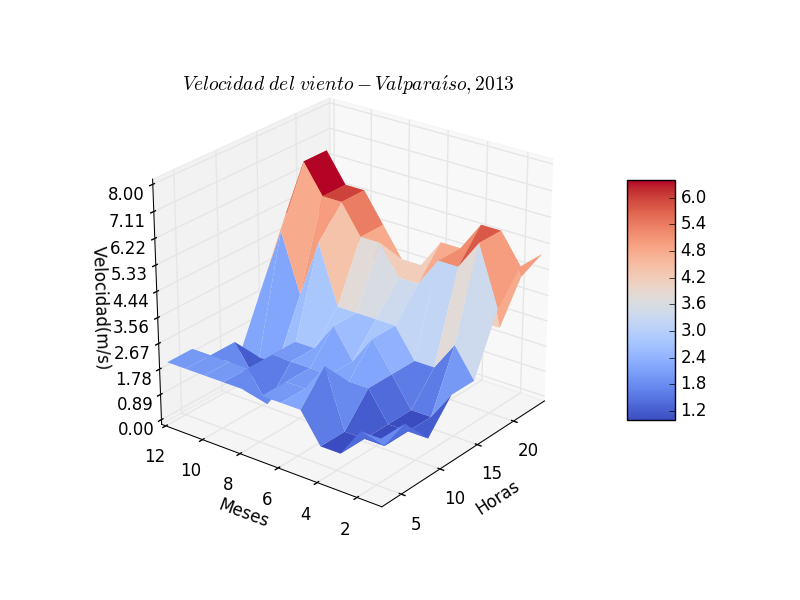
\includegraphics[height=75mm]{figures/3d_data_2013.png}
    \caption{Superficie datos Valparaíso 2013}
    \vspace{-.25cm}
    \caption*{Fuente: Elaboración Propia.}
    \label{fig:data_valpo_13}
\end{figure}
\begin{figure}[h!]
    \centering
    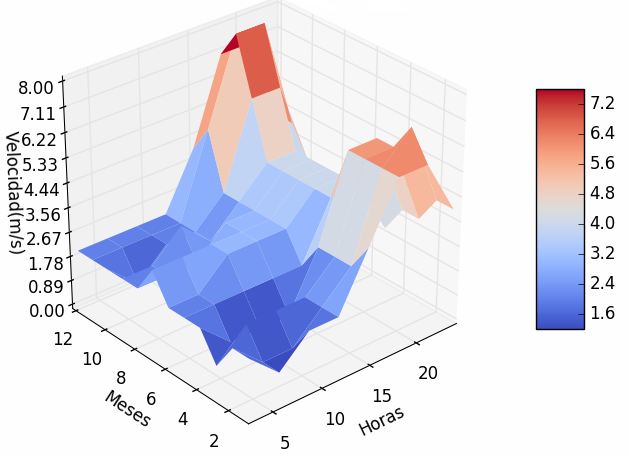
\includegraphics[height=75mm]{figures/3d_data_2014.png}
    \caption{Superficie datos Valparaíso 2014}
    \vspace{-.25cm}
    \caption*{Fuente: Elaboración Propia.}
    \label{fig:data_valpo_14}
\end{figure}
\begin{figure}[h!]
    \centering
    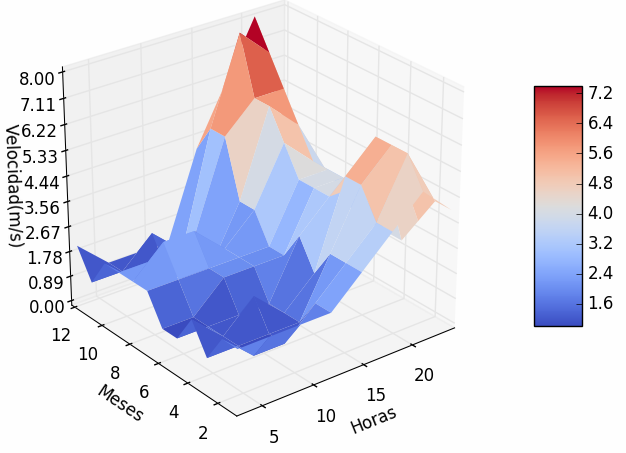
\includegraphics[height=75mm]{figures/3d_data_2015.png}
    \caption{Superficie datos Valparaíso 2015}
    \vspace{-.25cm}
    \caption*{Fuente: Elaboración Propia.}
    \label{fig:data_valpo_15}
\end{figure}
\begin{figure}[h!]
    \centering
    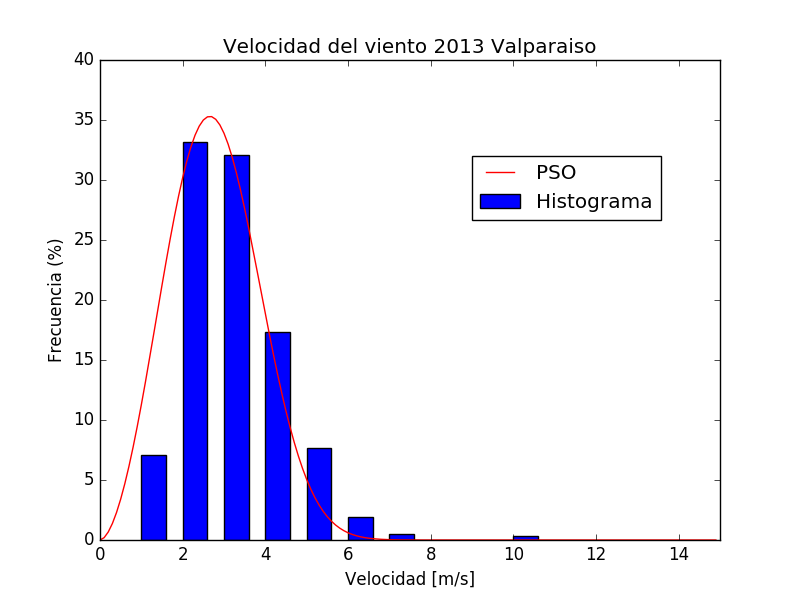
\includegraphics[height=75mm]{figures/result_2013.png}
    \caption{Ajuste con PSO a datos Valparaíso 2013}
    \vspace{-.25cm}
    \caption*{Fuente: Elaboración Propia.}
    \label{fig:pso_valpo_13}
\end{figure}
\begin{figure}[h!]
    \centering
    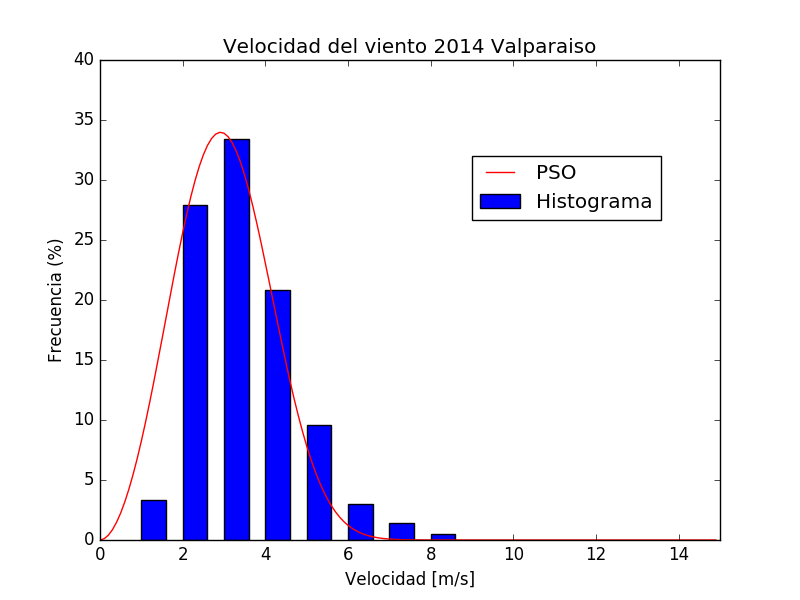
\includegraphics[height=75mm]{figures/result_2014.png}
    \caption{Ajuste con PSO a datos Valparaíso 2014}
    \vspace{-.25cm}
    \caption*{Fuente: Elaboración Propia.}
    \label{fig:pso_valpo_14}
\end{figure}
\begin{figure}[h!]
    \centering
    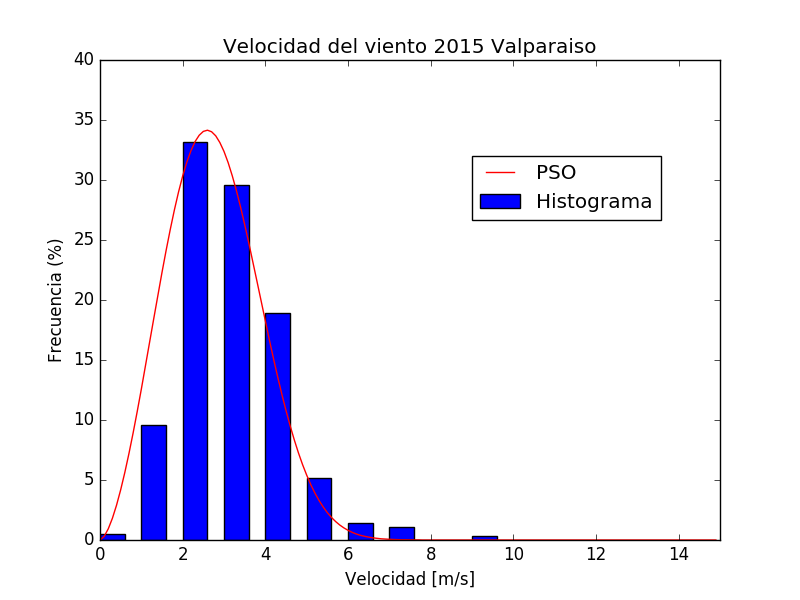
\includegraphics[height=75mm]{figures/result_2015.png}
    \caption{Ajuste con PSO a datos Valparaíso 2015}
    \vspace{-.25cm}
    \caption*{Fuente: Elaboración Propia.}
    \label{fig:pso_valpo_15}
\end{figure}

%Desde acá

\begin{figure}[h!]
    \centering
    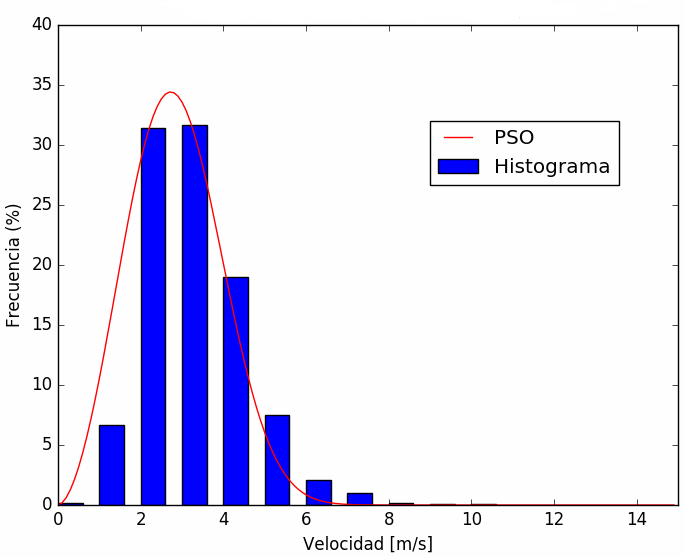
\includegraphics[height=75mm]{figures/result_13-14-15.png}
    \caption{Ajuste con PSO a datos Valparaíso 2015, 2014 y 2013}
    \vspace{-.25cm}
    \caption*{Fuente: Elaboración Propia.}
    \label{fig:pso_valpo_15_14_13}
\end{figure}
\begin{figure}[h!]
    \centering
    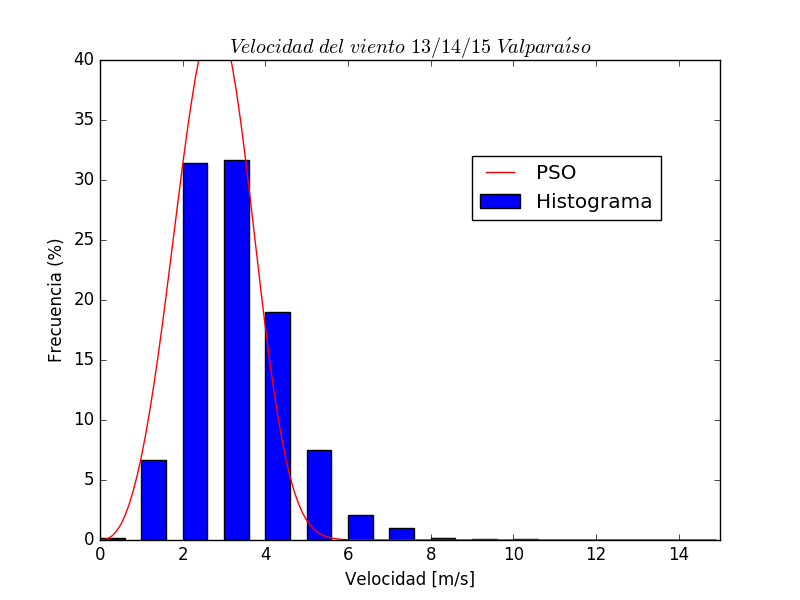
\includegraphics[height=75mm]{figures/result_13-14-15_low_quality.png}
    \caption{Ajuste con PSO a datos Valparaíso 2015, 2014 y 2013, baja calidad}
    \vspace{-.25cm}
    \caption*{Fuente: Elaboración Propia.}
    \label{fig:pso_valpo_15_14_13_lq}
\end{figure}
\begin{figure}[h!]
    \centering
    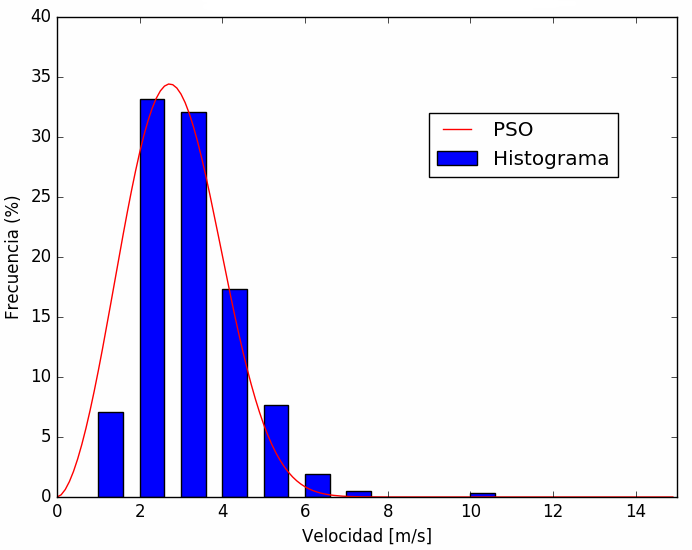
\includegraphics[height=75mm]{figures/result_2013_fit_all_data.png}
    \caption{Ajuste con PSO (Con todos los datos) a datos Valparaíso 2013}
    \vspace{-.25cm}
    \caption*{Fuente: Elaboración Propia.}
    \label{fig:pso_valpo_13_all_data}
\end{figure}
\begin{figure}[h!]
    \centering
    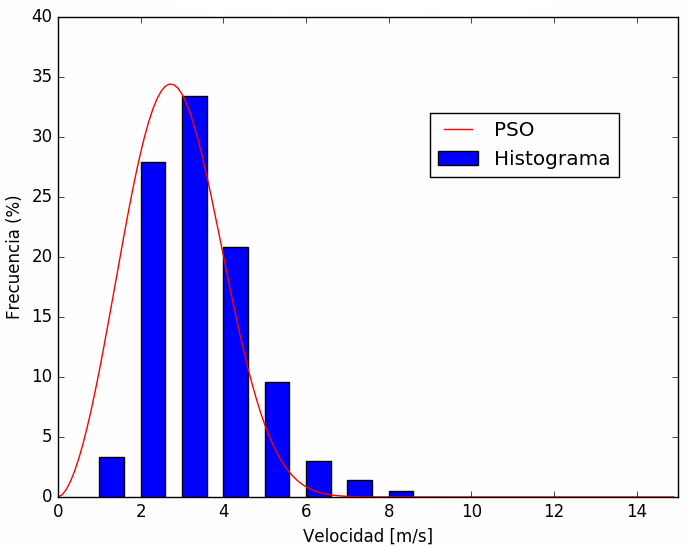
\includegraphics[height=75mm]{figures/result_2014_fit_all_data.png}
    \caption{Ajuste con PSO (Con todos los datos) a datos Valparaíso 2014}
    \vspace{-.25cm}
    \caption*{Fuente: Elaboración Propia.}
    \label{fig:pso_valpo_14_all_data}
\end{figure}
\begin{figure}[h!]
    \centering
    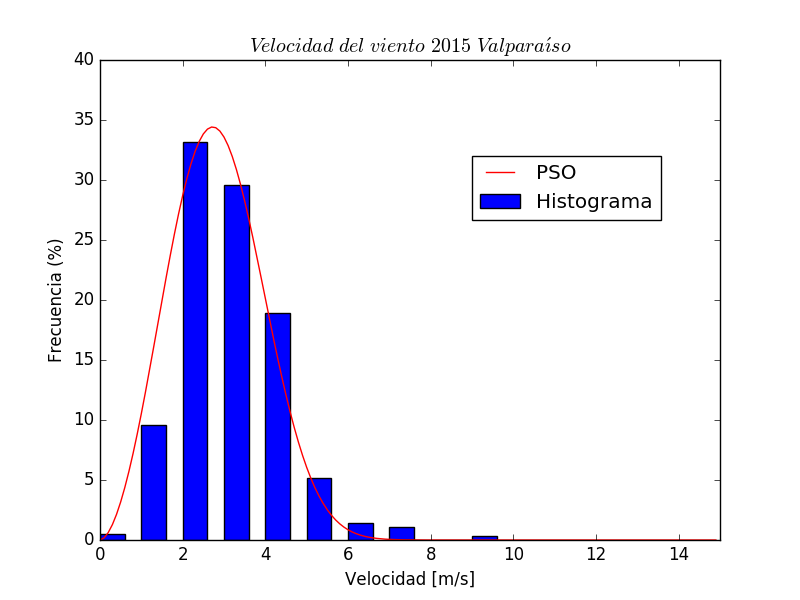
\includegraphics[height=75mm]{figures/result_2015_fit_all_data.png}
    \caption{Ajuste con PSO (Con todos los datos) a datos Valparaíso 2015}
    \vspace{-.25cm}
    \caption*{Fuente: Elaboración Propia.}
    \label{fig:pso_valpo_15_all_data}
\end{figure}
\begin{figure}[h!]
    \centering
    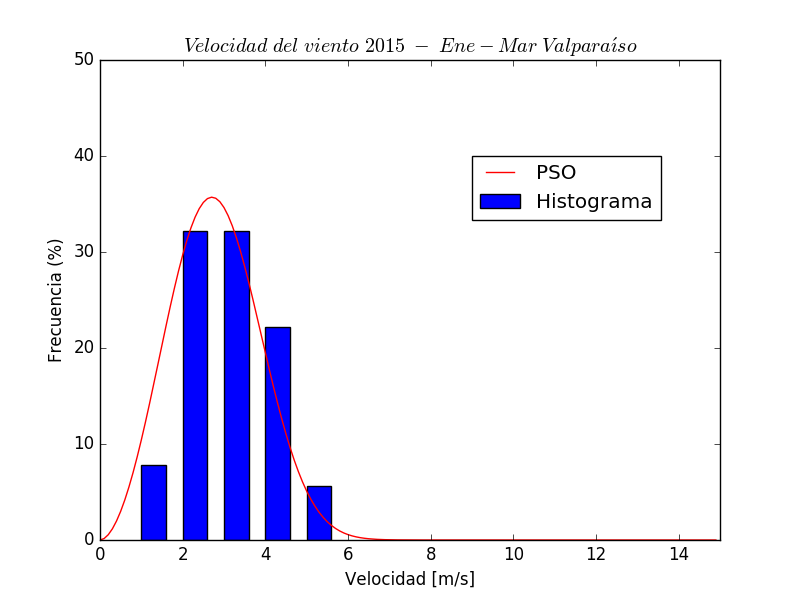
\includegraphics[height=75mm]{figures/result_2015_Ene-Mar.png}
    \caption{Ajuste con PSO a datos Valparaíso 2015, Enero - Marzo}
    \vspace{-.25cm}
    \caption*{Fuente: Elaboración Propia.}
    \label{fig:pso_valpo_15_ene_mar}
\end{figure}
\begin{figure}[h!]
    \centering
    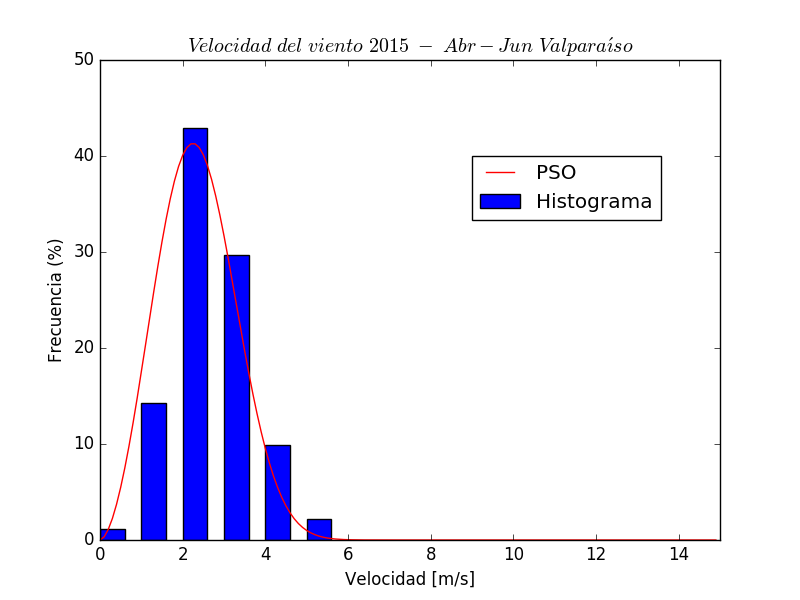
\includegraphics[height=75mm]{figures/result_2015_Abr-Jun.png}
    \caption{Ajuste con PSO a datos Valparaíso 2015, Abril - Junio}
    \vspace{-.25cm}
    \caption*{Fuente: Elaboración Propia.}
    \label{fig:pso_valpo_15_abr_jun}
\end{figure}
\begin{figure}[h!]
    \centering
    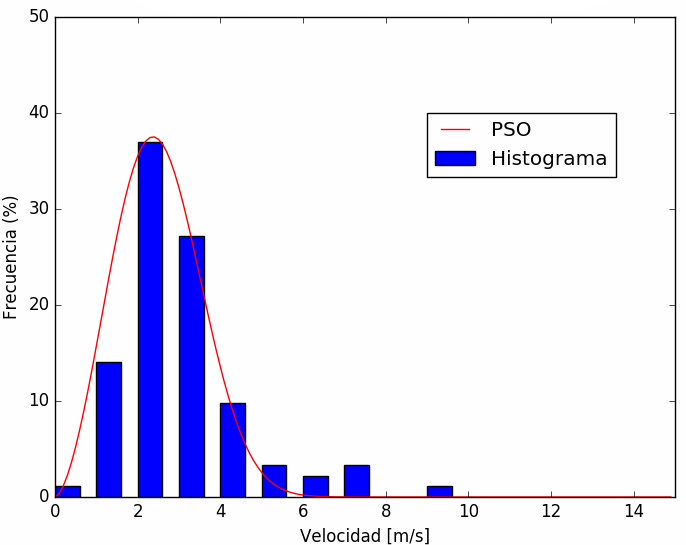
\includegraphics[height=75mm]{figures/result_2015_Jul-Sep.png}
    \caption{Ajuste con PSO a datos Valparaíso 2015, Julio - Septiembre}
    \vspace{-.25cm}
    \caption*{Fuente: Elaboración Propia.}
    \label{fig:pso_valpo_15_jul_sep}
\end{figure}
\begin{figure}[h!]
    \centering
    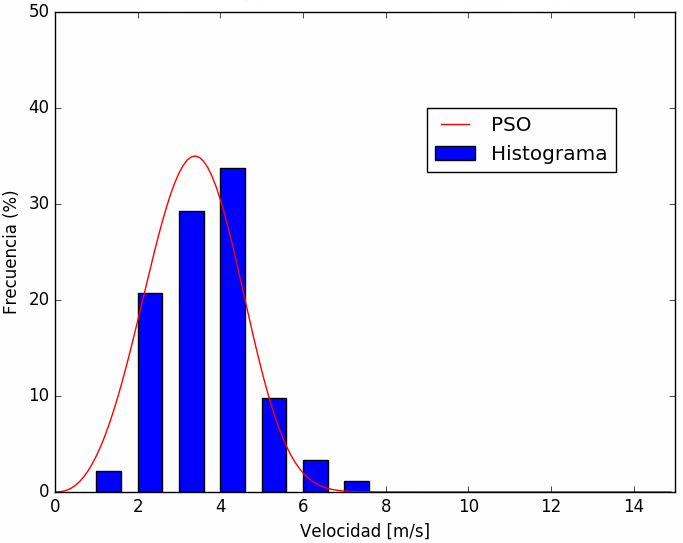
\includegraphics[height=75mm]{figures/result_2015_Oct-Dic.png}
    \caption{Ajuste con PSO a datos Valparaíso 2015, Octubre - Diciembre}
    \vspace{-.25cm}
    \caption*{Fuente: Elaboración Propia.}
    \label{fig:pso_valpo_15_oct_dic}
\end{figure}
\begin{figure}[h!]
    \centering
    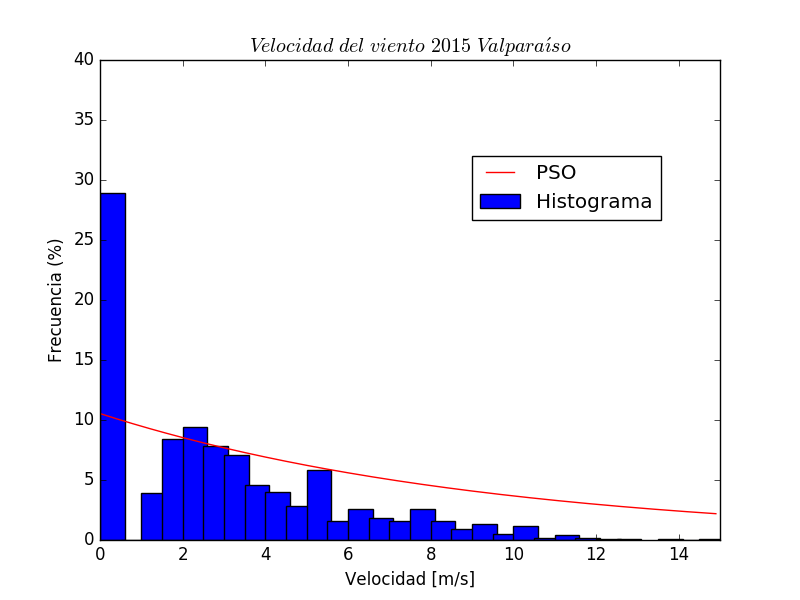
\includegraphics[height=75mm]{figures/result_2015_all_data.png}
    \caption{Ajuste con PSO a datos (cifras puras) Valparaíso 2015, 2014, 2013}
    \vspace{-.25cm}
    \caption*{Fuente: Elaboración Propia.}
    \label{fig:pso_valpo_15_oct_dic}
\end{figure}


\begin{table}[htb!]
    \centering
    \caption{Tabla de tests estadísticos}
    \label{table:stadistical_tests}
    %\resizebox{\columnwidth}{!}{
    \begin{tabular}{|c|c|c|c|c|c|c|}
        \hline
        \textbf{Método} & \textbf{Período} & \textbf{k} & \textbf{c} & \textbf{RMSE} & \textbf{r} & \textbf{RB}\\
        \hline
        PSO & 2013 & 2.78 & 3.12 &0.0226585230791 & 0.984353070415 & 0.00197971468299\\
        PSO & 2014 & 2.91 & 3.37 &0.0232779965263 & 0.982087745069 & 0.000754465101398\\
        PSO & 2015 & 2.65 & 3.10 &0.0164721412159 & 0.992323803649 & 0.00302918178445\\
        \hline
        PSO (Intento 1) & 2015-14-13 & 3.47 & 3.07 & 0.0360794587206 & 0.975240385258 & 0.000411212628513\\
        PSO (Intento 2) & 2015-14-13 & 2.78 & 3.20 & 0.016175531561 & 0.994989105807 & 0.00190916669626\\
        \hline
        PSO (Intento 2) & 2013 & 2.78 & 3.20 & 0.0240448436122 & 0.981963054492 & 0.00192186034284\\
        PSO (Intento 2) & 2014 & 2.78 & 3.20 & 0.0301463089474 & 0.970662237238 & 8.89024791609e-05\\
        PSO (Intento 2) & 2015 & 2.78 & 3.20 & 0.0202342934641 & 0.98662798667 & 0.00192175053173\\
        \hline
        PSO & Ene-Mar & 2.85 & 3.15 & 0.0230380400157 & 0.982158006469 & 0.00641888742608\\
        PSO & Abr-Jun & 2.76 & 2.65 & 0.0204300909755 & 0.993857185938 & 0.00303620481316\\
        PSO & Jul-Sep & 2.66 & 2.83 & 0.0251002816356 & 0.985858767021 & 0.00443453471038\\
        PSO & Oct-Dic & 3.40 & 3.75 & 0.0260278634297 & 0.978479679326 & 0.000716653529598\\
        \hline 
        PSO (datos brutos) & 2015 & 1.00 & 9.49 & 0.0451794472583 & 0.751732944794 & 0.676094670465\\ 
    \end{tabular}
    %}   
\end{table}
\pagebreak
\subsection{Conclusiones}
De los gráficos expuestos anteriormente, es apreciable que en Valparaíso las máximas velocidades de viento aparecen entre Septiembre y Febrero aproximadamente, entre las 18:00 y las 23:00 hrs, sin embargo, observando los histogramas, se observa una concentración entre los 2 y 4 $[m/s]$ de velocidad, por lo que se puede concluir que las máximas de viento son esporádicas en la zona.\\ 
Si bien los resultados conseguidos no son de la misma calidad que los mostrados en el trabajo de Carneiro et al. \cite{Carneiro15}, el ajuste conseguido por el PSO es bueno y bastante cercano en precisión a los del trabajo citado, con una correlación entre del $99\%$ para el año 2015 y $98\%$ para los años 2013 y 2014, lo cual confirma que el \emph{Particle Swarm Optimization} es una excelente alternativa a los métodos numéricos tradicionales, no sólo desde el punto de vista de calidad de solución, sino que también, en simplicidad de implementación.\\
Con los parámetros $k$ y $c$ obtenidos se puede fácilmente replicar el modelo para los datos del viento de Valparaíso. Basta con definir la distribución de Weibull en base a estos.\\
Para trabajo futuro, queda extraer cualquier información posible desde el punto de vista estadístico de los modelos generados con el uso del PSO. Preguntas como, ¿Cuál es la probabilidad de que la velocidad del viento sea mayor a 3.5 $[m/s]$? ó ¿Cuál es la esperanza de velocidad de viento para hoy?, pueden ser fácilmente respondidas ajustando em modelo a la sección de datos requerida (diaria, mensual, anual, etc), con una alta confiabilidad.  